\documentclass{report}
\usepackage[utf8]{inputenc}
\usepackage[francais]{babel}
\usepackage[T1]{fontenc}
\usepackage{lmodern}
\usepackage{textcomp}
\usepackage{listings}
\usepackage{graphicx}
\usepackage{hyperref}
\usepackage{titlesec}
\usepackage{tcolorbox}
\usepackage{amsmath}
\usepackage{color}
\usepackage{multirow}
\setcounter{tocdepth}{5}
\setcounter{secnumdepth}{4}
\definecolor{dkgreen}{rgb}{0,0.6,0}
\definecolor{gray}{rgb}{0.5,0.5,0.5}
\definecolor{mauve}{rgb}{0.58,0,0.82}
\definecolor{gray}{rgb}{0.4,0.4,0.4}
\definecolor{darkblue}{rgb}{0.0,0.0,0.6}
\titleformat{\paragraph}
{\normalfont\normalsize\bfseries}{\theparagraph}{1em}{}
\titlespacing*{\paragraph}
{0pt}{3.25ex plus 1ex minus .2ex}{1.5ex plus .2ex}
\renewcommand{\thesection}{\Roman{section}}
\hypersetup{
    colorlinks=true,
    linkcolor=black,
    filecolor=magenta,
    urlcolor=cyan,
}
\lstnewenvironment{cc}
{
\lstset{frame=tblr,
  language=C,
  aboveskip=3mm,
  belowskip=3mm,
  showstringspaces=false,
  columns=flexible,
  basicstyle={\small\ttfamily},
  numbers=none,
  numberstyle=\tiny\color{gray},
  keywordstyle=\color{blue},
  commentstyle=\color{dkgreen},
  stringstyle=\color{mauve},
  breaklines=true,
  breakatwhitespace=true,
  tabsize=3
}}
{}

\begin{document}
\title{
  \begin{minipage}\linewidth
      \centering
      
\includegraphics[width=40mm]{resources/01.png}\vskip 20pt
      Projet AOA sujet 10 : Phase 2
      \vskip 5pt
      \author{
        ALEXANDRE Julien \\
        \texttt{julien.alexandre@isty.uvsq.fr}
      \and
        VIRLOGEUX Marin \\
        \texttt{marin.virlogeux@isty.uvsq.fr}
      \and
        LEDOYEN Paul \\
        \texttt{paul.ledoyen@isty.uvsq.fr}
      \and
        DRISSI Mohamed Reda \\
        \texttt{reda-mohamed@isty.uvsq.fr}
      }
    \end{minipage}
}
\maketitle
\newpage
\tableofcontents
\newpage
\section{Introduction}
 \subsection{Objectifs}
  	L'objectif de ce projet est d'étudier un noyau de code et d'optimiser son code. Nous traitons ici la phase II de ce projet qui consiste en
  	\begin{itemize}
  	\item mesurer la performance du noyau avec différentes optimisations du code de la fonction \texttt{baseline}
    \item Utiliser les outils MAQAO et likwid pour trouver ce qui reste à optimiser
  	\item trouver d'autres méthodes d'optimisation pertinentes
	  \item Noter les différences de performances ainsi que les étapes suivies pour les obtenir
    \item Optimiser à l'aide de flags de compilation ou autres compilateurs
	  \item Essayer OpenMP et d'autres compilateurs
  	\end{itemize}
  \subsection{Spécifications de la machine utilisée}
  Nous avons traité les différents cas sur la même machine pour conserver une certaine constance dans les mesures effectuées.
    \begin{itemize}
      \item CPU : \href{https://ark.intel.com/products/88195/Intel-Core-i7-6700K-Processor-8M-Cache-up-to-4_20-GHz}
        {intel core i7 6700K 4.0GHZ 4 physical cores, 8 logical(HyperThreading©) turbo boost off}
      \item RAM : Corsair CMK16GX4M2B3000C15 Vengeance LPX 16GB DDR4 3000MHz C15 XMP 2.0
      \item Stockage : \href{http://downloadcenter.samsung.com/content/UM/201711/20171115103115156/Samsung_SSD_850_PRO_Data_Sheet_Rev_3.pdf}
          {Samsung 850 PRO SSD 512GB}
    \end{itemize}
    \subsection{Système}
      \begin{itemize}
      \item OS : Debian 9.4 Stretch (stable) x86\_64
      \item Kernel :  4.9.0-6-amd64
      \item GCC\textsuperscript \textcopyleft   : 6.3.0 20170516 (Debian 6.3.0-18+deb9u1)
      \item ICC : 18.0.1 20171018
      \item \href{http://www.openmp.org/wp-content/uploads/openmp-4.5.pdf}{openMP: 4.5}
    \end{itemize}
  \subsection{Topologie du système}
    \begin{figure}[ht!]
      \centering
      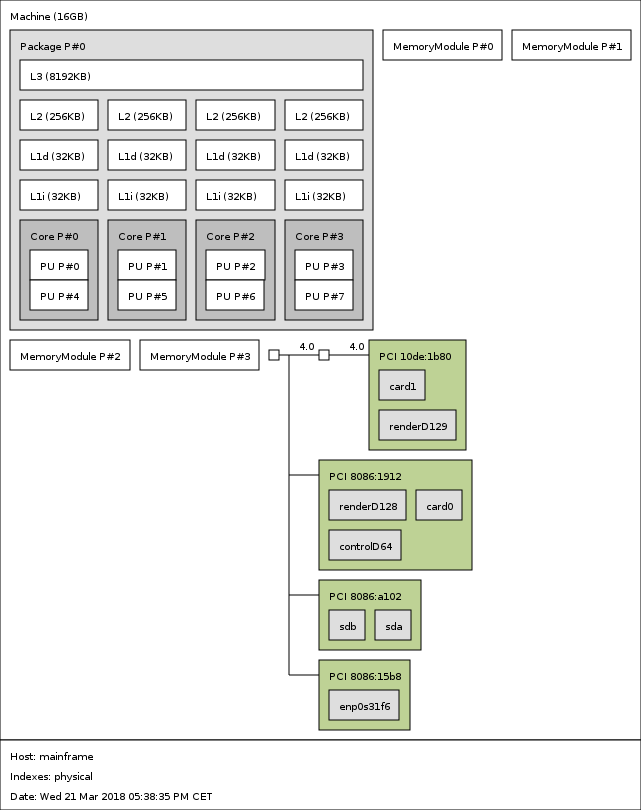
\includegraphics[scale=0.35]{resources/lstopo.png}
      \caption{Topologie générée par \href{https://manpages.debian.org/jessie/hwloc/lstopo.1.en.html}{lstopo}}
    \end{figure}
  \newpage
\section{Optimisation du code}
  \subsection{Protocole }
    Nous allons à chaque itération mesurer les performances à l'aide de la même méthode utilisée en phase 1
    (rdtsc), le nombre de cycles par itération donne des valeurs significatives et lisible pour l'humain.
    Afin d'éviter l'interférence et limiter la dépendance sur le fonctionnement de l'OS, nous allons
    utlisier \texttt{taskset} puis nous allons redémarrer notre machine entre chaque 2 mesures, un
    cronjob s'occuppe de lancer la prochaine mesure et pendant ces mesures, la machine démarre
    en mode terminal et se log automatiquement.
    \\La procédure étant complètement autonome, les résultats seront stockés dans des tsv.
    Puis nous garderons la médiane des valeurs à chaque fois, nous allons ensuite générer des
    graphiques depuis ces tsv.
    Pour cette partie nous allons nous contenter de \texttt{gcc -O2} pour la compilation.
  \subsection{Choix des paramètres}
    Nous allons exécuter notre code en L1 pour éviter les goulets d'étranglement causé par la lenteur
    de la RAM, nous avons utilisé $50$ dans la phase 1 pour L1, ici nous allons utilisé $48$ pour le déroulement de la boucle
    . Le nombre de warmup sera à 20 pour la première méta repétition puis à 3 pour le reste puisque
    d'après la phase I nous n'avons pas besoin de plus. \\
    Le nombre de méta répétitions demandé par le prof est 31, cependant vu que la machine est assez
    rapide et que la taille du tableau est assez petite, nous pouvons nous permettre de l'élever à 200
    comme ça la médiane sera améliorée.
    Donc :
    \begin{center}
      \begin{tabular}{ | l | c |  }
        \hline
        Taille & 48  \\ \hline
        Warmup & 20 puis 3  \\ \hline
        MetaRep & 200  \\ \hline
      \end{tabular}
    \end{center}
  \subsection{Code initial}
  \subsubsection{Code}
  \begin{cc}
    float baseline(int n,double a[n][n])
    {
        int i,j;
        float s=0.0;
        for(j=0;j<n;j++)
            for(i=0;i<n;i++)
                s += a[i][j];
        return s;
    }
  \end{cc}
  \subsubsection{Performance}
  Nous trouvons en médiane : $13.986465$ cycles par itération.
  \begin{figure}[ht!]
    \centering
    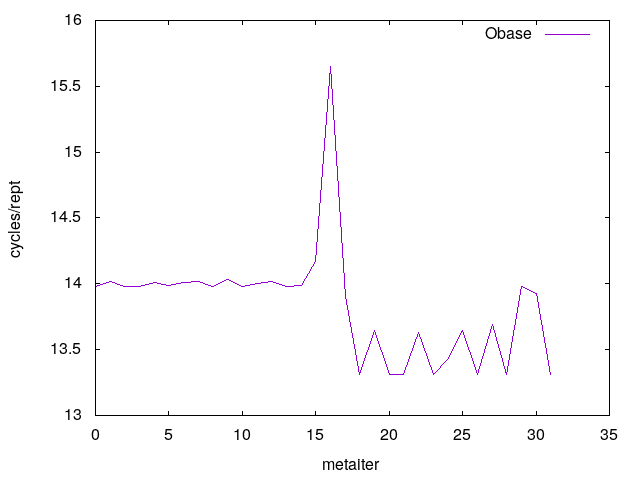
\includegraphics[scale=0.45]{../metarep/Obase.png}
    \caption{Résultat du du code initial}
  \end{figure}
  \subsubsection{Résultats MAQAO}
  D'après le résultat de \texttt{cqa} nous devons utiliser les même types pour nos variables et
  constantes, en effet \texttt{cqa} trouve des opérations de conversion très coûteuses.
  \begin{verbatim}
    Conversion instructions
    -----------------------
    Detected expensive conversion instructions (typically from/to single/double precision).
    - CVTSS2SD: 1 occurrences
    - CVTSD2SS: 1 occurrences
  \end{verbatim}
  \subsection{Conversion de types}
  \subsubsection{code}
  \begin{cc}
    double baseline(int n,double a[n][n])
    {
        int i,j;
        double s=0.0;
        for(j=0;j<n;j++)
            for(i=0;i<n;i++)
                s += a[i][j];
        return s;
    }
  \end{cc}
  \subsubsection{Performance}
  Nous trouvons en médiane : $3.944666$ cycles par itération.\\
  Ce qui veut dire un speed up très important par rapport au code initial de :
  \begin{center}
      $3.546$
  \end{center}
  \begin{figure}[ht!]
    \centering
    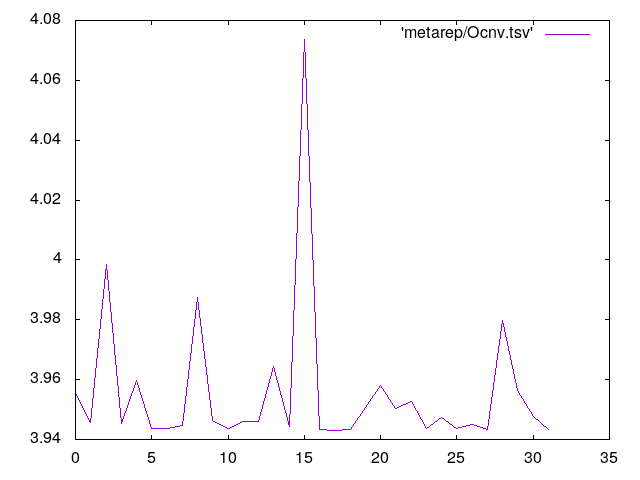
\includegraphics[scale=0.45]{../metarep/Ocnv.png}
    \caption{Résultat de l'optimisation par conversion des types}
  \end{figure}
  \subsubsection{Résultats MAQAO}
  D'après \texttt{cqa} il faut que nous changeant l'ordre d'accès à la mémoire, et accèder en lignes
  plutôt qu'en colonne, cela nous évitera le grand nombre de cache misses auquel on a affaire.
  \begin{verbatim}
    * If your arrays have 2 or more dimensions, check whether elements are accessed contiguously and,
    otherwise, try to permute loops accordingly:
    C storage order is row-major: for(i) for(j) a[j][i] = b[j][i]; (slow, non stride 1) =>
    for(i) for(j) a[i][j] = b[i][j]; (fast, stride 1)
    * If your loop streams arrays of structures (AoS), try to use structures of arrays instead (SoA):
    for(i) a[i].x = b[i].x; (slow, non stride 1) => for(i) a.x[i] = b.x[i]; (fast, stride 1)

  \end{verbatim}


  \subsection{Accès par lignes}
  \subsubsection{code}
  \begin{cc}
    float baseline(int n,float a[n][n])
    {
        int i,j;
        float s=0.0f;
        for(j=0;j<n;j++)
            for(i=0;i<n;i++)
                s += a[j][i];
        return s;
    }
  \end{cc}
  \subsubsection{Performance}
  Nous trouvons en médiane : $3.931523$ cycles par itération.\\
  Ce qui veut dire un speed up très faible par rapport à l'optimisation précédente de :
  \begin{center}
      $1.004$
  \end{center}
  \begin{figure}[ht!]
    \centering
    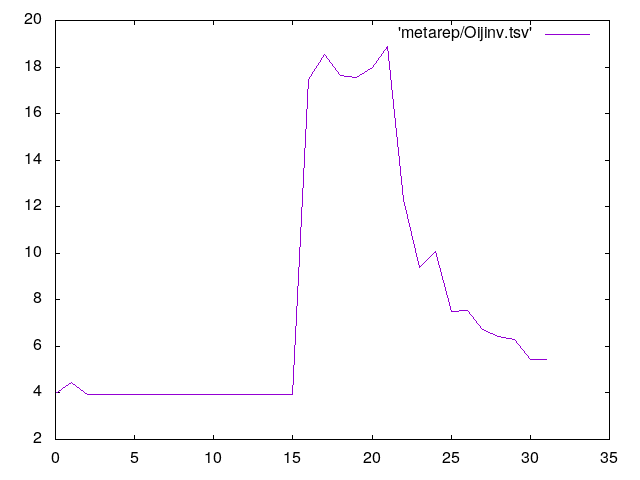
\includegraphics[scale=0.45]{../metarep/Oijinv.png}
    \caption{Résultat de l'accès en lignes}
  \end{figure}
  \subsubsection{Résultats MAQAO}
  Nous allons essayer de dérouler la boucles manuellement puisque ne nous pouvons pas utiliser
  des flags.
  \begin{verbatim}
    Unroll opportunity
    ------------------
    Loop body is too small to efficiently use resources.
    Workaround(s):
    Unroll your loop if trip count is significantly higher than target unroll factor. This can be done
    manually. Or by recompiling with -funroll-loops and/or -floop-unroll-and-jam.
  \end{verbatim}

  \subsection{Déroulement de boucles}
  \subsubsection{code}
  \begin{cc}
    float baseline(int n,float a[n][n])
    {
        int i,j;
        float s=0.0f,t=0.0f,u=0.0f,v=0.0f,w=0.0f,x=0.0f,y=0.0f,z=0.0f;
        for(j=0;j<n;j++)
        for(i=0;i<n;i=i+8)
        {
              s += a[j][i];
              t += a[j][i+1];
              u += a[j][i+2];
              v += a[j][i+3];
              w += a[j][i+4];
              x += a[j][i+5];
              y += a[j][i+6];
              z += a[j][i+7];

        }

        return s+t+u+v+w+x+y+z;
    }
  \end{cc}
  \subsubsection{Performance}
  Nous trouvons en médiane : $0.572415$ cycles par itération.\\
  Ce qui veut dire un speed up très important par rapport à l'optimisation précédente de :
  \begin{center}
      $6.868$
  \end{center}
  \begin{figure}[ht!]
    \centering
    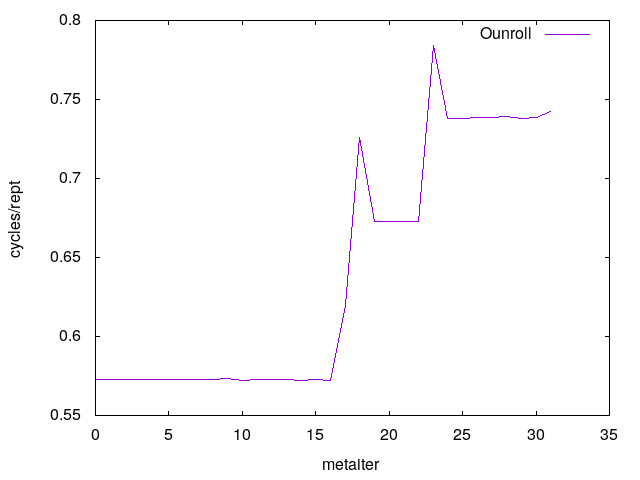
\includegraphics[scale=0.45]{../metarep/Ounroll.png}
    \caption{Résultat du déroulement de la boucle}
  \end{figure}
  \subsubsection{Résultats MAQAO}
  En déroulant la boucle en 4 étapes par itérations nous obtenons un speed up d'environ $3.961$.
  En exécutant \texttt{cqa} nous trouvons que nous pouvons encore optimiser. Donc nous déroulons
  en 8 étapes, qui est le résultat que nous gardons, parce qu'au delà de 8, nous mettons trop de
  stress sur l'unité d'addition FP.
  \textt{cqa} qu'il y a un goulet d'étranglement :
  \begin{verbatim}
    Bottlenecks
    -----------
    Performance is limited by writing data to caches/RAM (the store unit
    is a bottleneck).
  \end{verbatim}
  Ce n'est pas grave, car notre itération même si coûteuse nous permet de diviser le nombre
  total d'itérations par 8.\\
  Après cela, \texttt{cqa} ne nous donne pas d'autres indices sur l'amélioration du code à part ce
  qui a déjà été effectué, donc nous passons à l'étape suivante qui est d'utiliser les optimisations
  que nous avons trouvé en Phase I.

  \subsection{Optimisation de compilation}
  \subsubsection{\texttt{-fast}}
  Nous allons utiliser les meilleurs optimisations trouvé en Phase I :
  \begin{verbatim}
    icc -Wall -fast -opt-prefetch -unroll-aggressive
  \end{verbatim}
  \paragraph{Performance}
  Nous trouvons en médiane : $0.000056$ cycles par itération.\\
  Ce qui veut dire un speed up étonnant par rapport au code optimisé :
  \begin{center}
      $10221.696$
  \end{center}
  \begin{figure}[ht!]
    \centering
    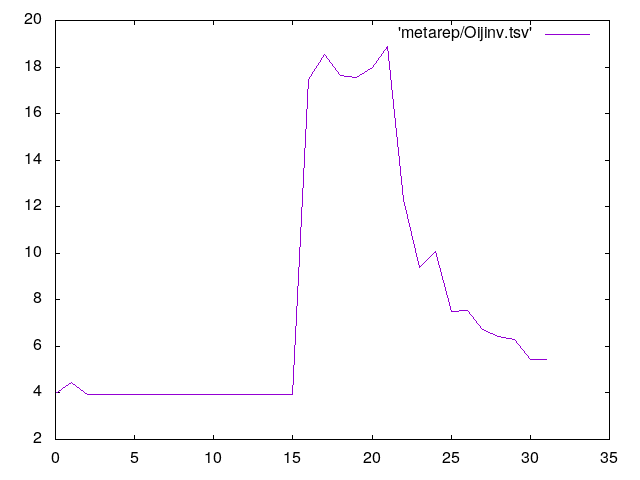
\includegraphics[scale=0.45]{../metarep/Oijinv.png}
    \caption{Résultat du du code initial}
  \end{figure}
  \paragraph{Résultats MAQAO}
  Nous ne pouvons rien dire, \texttt{cqa} retourne :
  \begin{verbatim}
    Info: No function matches the pattern baseline in the binary ./Ofun_i
  \end{verbatim}
  Ceci est dû au flag \texttt{-ipo} qui est imprévisible et change forcèment
  soit l'emplacement de la boucle soit la boucle elle même, c'est pour cela que nous n'allons pas l'utiliser
  \subsubsection{\texttt{-Ofast}}
  Le flag \texttt{Ofast} génère un temps de $0.713548$ contre $0.571706$ en \texttt{O2}. Puis Nous remarquons
  en testons \texttt{O3} (qui donne le même résultat que \texttt{O2}) que le problème vient de \texttt{-ffast-math}
  couplé à \texttt{O3}. \\
  En effet \texttt{-O3 -ffast-math} vectorise partiellement notre boucle :
  \begin{verbatim}
    Your loop is PARTIALLY VECTORIZED and could benefit from full vectorization.
    By fully vectorizing your loop, you can lower the cost of an iteration from
    4.00 to 2.00 cycles (2.00x speedup).
  \end{verbatim}
  Mais ce gain ne vaut pas le coup puisqu'il coûte à peu près $20\%$ de
  la performance obtenu avec le flag \texttt{-O2} qui lui ne vectorise pas :
  \begin{verbatim}
    Your loop is NOT VECTORIZED and could benefit from vectorization.
    By vectorizing your loop, you can lower the cost of an iteration
    from 4.00 to 0.50 cycles (8.00x speedup).
  \end{verbatim}
  %%%%%%%%%%%%%%%%%%%%%%%%%%%%%%%%%%%%%%%%%%%%%%%%%%%%%%%%%%%%%%%%%%%%%%%%%
  %%%%%%%%%%%%%%%%%%%%%%%%%%%%%%%%%%%%%%%%%%%%%%%%%%%%%%%%%%%%%%%%%%%%%%%%%
  \subsubsection{\texttt{icc}}
  Nous trouvons avec \texttt{icc -O3} un temps de $0.630128$ donc c'est une
  perte par rapport à \texttt{gcc -O3} qui trouve $0.569972$.\\
  Nous trouvons avec \texttt{icc -O2} un temps de $0.513700$ donc c'est une
  perte par rapport à \texttt{gcc -O2} qui trouve $0.572750$. Soit un gain
  de $1.115$\\
  Donc la meilleure config sera de \texttt{icc -O2}
  Par contre en essayant \texttt{-march=skylake} nous trouvons l'inverse, soit
  un résultat similaire à l'addition de \texttt{-ffast-math}.
  \texttt{gcc -O2 -march=skylake} donne $0.582897$
  \texttt{icc -O2 -xHost} donne $0.770447$
  \texttt{gcc -O3 -march=skylake} donne $0.696146$
  \texttt{icc -O3 -xHost} donne $0.711994$
  Nous resterons alors sur \texttt{icc -O2}
  %%%%%%%%%%%%%%%%%%%%%%%%%%%%%%%%%%%%%%%%%%%%%%%%%%%%%%%%%%%%%%%%%%%%%%%%%
  %%%%%%%%%%%%%%%%%%%%%%%%%%%%%%%%%%%%%%%%%%%%%%%%%%%%%%%%%%%%%%%%%%%%%%%%%
  \subsection{Optimisation OpenMP}
  \subsubsection{code}
  \begin{cc}
    #define N_THRD 8
    #include <omp.h>
    float baseline(int n,float a[n][n])
    {
        int i,j;
        float s=0.0f,t=0.0f,u=0.0f,v=0.0f,w=0.0f,x=0.0f,y=0.0f,z=0.0f;
        #pragma omp parallel for
        for(j=0;j<n;j++)
          for(i=0;i<n;i=i+8)
          {
                s += a[j][i];
                t += a[j][i+1];
                u += a[j][i+2];
                v += a[j][i+3];
                w += a[j][i+4];
                x += a[j][i+5];
                y += a[j][i+6];
                z += a[j][i+7];
          }

        return s+t+u+v+w+x+y+z;
    }
  \end{cc}
  \subsubsection{Performance}
  Nous trouvons en médiane : $31.620731$ cycles par itération.\\
  Ce nombre est étonnant, peut-être que la création des threads + la synchronisation
  des accès aux données partagées soit beaucoup plus coûteuse pour openMP que ça cache le gain obtenu.
  Nous allons exécuter le code avec et sans openMP avec une taille de $1000$ pour éviter ce problème.
  Nous trouvons :
  \begin{center}
    \begin{tabular}{ | l | c | c | }
      \hline
      Exec    & L1          & RAM         \\ \hline
      Ofun\_i & $0.000056$  & $0.000001$  \\ \hline
      Omp     & $31.620731$ & $0.941170$  \\ \hline
    \end{tabular}
  \end{center}
  Nous remarquons que malgré ce que nous avons essayé, l'optimisation d'openMP ne fait que rendre
  le code plus lent, parce que le code n'a pas été vectorisé.
  Nous essayons de comprendre la cause de ce problème à l'aide de \texttt{-qopt-report} de icc.
  D'après le rapport, la boucle interne n'a pas pu être parallélisé, donc nous allons réessayer
  en enlevant cette contrainte.\\
  Effectivement après avoir enlevé le pragma interne, le compilateur réussit à vectoriser la boucle.\\
  Cependant le gain obtenu, est inférieur au coût.\\
  Nous allons ensuite essayer plusieurs combinaisons pour trouver ce qui ne va pas.
  %%%%%%%%%%%%%%%%%%%%%%%%%%%%%%%%%%%%%%%%%%%%%%%%%%%%%%%%%%%%%%%%%%%%%%%%%
  %%%%%%%%%%%%%%%%%%%%%%%%%%%%%%%%%%%%%%%%%%%%%%%%%%%%%%%%%%%%%%%%%%%%%%%%%%%
  O2 openmp  avec 1 thread: 0.568937 (même que sans openmp)
  O2 openmp  avec 2 thread: 18.833143 (plus lent que la version basique)
  O3 openmp  avec 2 threads: 19.111582
  %%%%%%%%%%%%%%%%%%%%%%%%%%%%%%%%%%%%%%%%%%%%%%%%%%%%%%%%%%%%%%%%%%%%%%%%%
  %%%%%%%%%%%%%%%%%%%%%%%%%%%%%%%%%%%%%%%%%%%%%%%%%%%%%%%%%%%%%%%%%%%%%%%%%%%
  \begin{figure}[ht!]
    \centering
    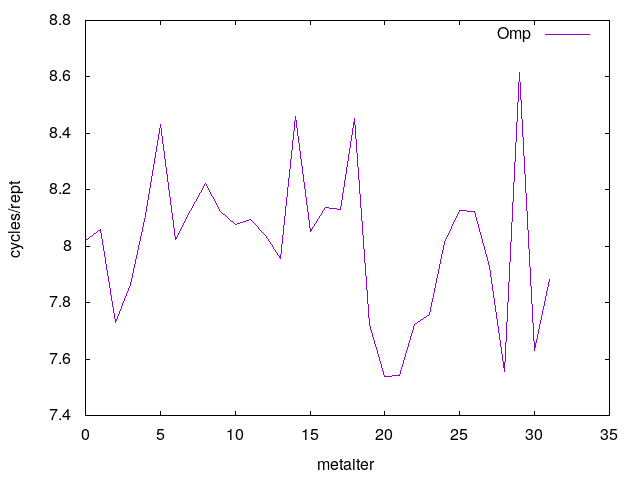
\includegraphics[scale=0.45]{../metarep/Omp.png}
    \caption{Résultat de l'optimisation OpenMP}
  \end{figure}
  \subsubsection{Résultats MAQAO}
  La sortie de \texttt{cqa} est similaire à la précédente.

  %%%%%%%%%%%%INSERT GRAPHIC%%%%%%%%%%%%%%%%%%%%

\end{document}
